\chapter{基于OpenMP的形态学图像处理}
\section{实验目的与要求}
\begin{enumerate}
    \item 掌握使用OpenMP进行并行编程设计和性能优化的基本原理和方法
    \item 使用OpenMP实现形态图像处理操作的并行算法
    \item 对程序执行结果进行简单的分析和总结
    \item 将其与Lab2的结果进行比较
\end{enumerate}

\section{算法描述}
\par 使用OpenMP进行并行计算与使用pthread进行并行计算的算法原理几乎一样,只不过OpenMP由编译器进行底层实现,使用for循环进行包装,且主线程不是空闲的,而是也参与计算。而pthread则需要人工进行底层的编写。使用OpenMP的关键部分代码如下:
\inputCodeSetLanguage{c++}
\begin{lstlisting}
#pragma omp parallel for num_threads(threadNum) schedule(dynamic, 2)
for(int i=0; i < workNum; ++i){
    // Code equvilent to calling ErodeAndDilate(blk, kernel_e, kernel_d)
}
\end{lstlisting}
\par OpenMP caluse中的schedule(dynamic, 2)将所有的人物按照2个一组进行分组,而每个线程领取一组任务、执行完成后在领取下一组可能的任务,从而避免了由于静态调度以及线程执行时间不等带来的CPU空闲。

\section{实验方案}
\par 由于算法与pthread基本相同,因此可以在pthread的实现上进行修改,将pthread中的线程竞争调度改为使用openmp directive包装的for循环,并在编译条件中去除-lpthread,加上-fopenmp即可。
\par 在运行时,通过多次调节参数并进行重复实验,得到一侧较优的参数,然后将这个参数与phtread实现进行对比,观察OpenMP实现与pthread实现的区别。

\section{实验结果与分析}
\par 功能上,OpenMP能够正确的处理图片并给出与串行处理相同的结果。性能上,使用4线程、分块大小128时程序的运行结果如图\ref{fig:ompOutput}所示。三次测试平均结果为12.63s,相对于串行程序加速比为\(44.2\div 12.63 = 3.49\),与同条件下的pthread实现比起来加速比要低不少,这是由于OpenMP需要进行环境的初始化,且其调度过程没有特别为底层实现的pthread程序优化,因此pthread实现的并行程序性能较为优秀。
\begin{figure}[htpb]
    \centering
    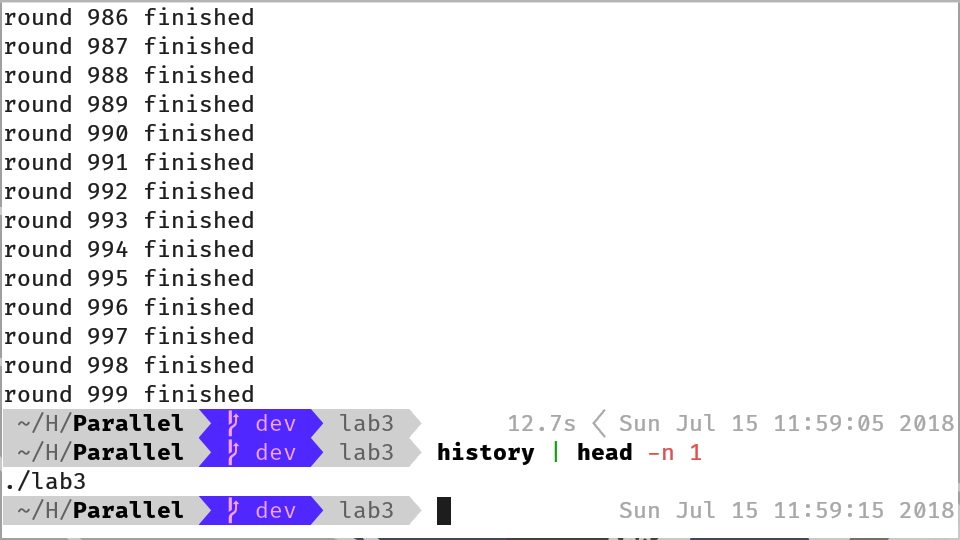
\includegraphics[width=0.9\linewidth]{ompOutput.png}
    \caption{使用OpenMP进行处理的输出}
    \label{fig:ompOutput}
\end{figure}

\par 加速比随线程数量变化如图\ref{fig:ompTrend}所示,其中实线部分为使用OpenMP的程序,而虚线部分为上述使用pthread的程序。从图中可以看出,使用OpenMP和使用pthread程序的性能随着线程数量的变化趋势是一样的,因为其算法本质上是相同的。而使用OpenMP的程序在同样的情况下总是比使用pthread的程序要慢一些,这也是由于OpenMP并不是一个针对特殊程序的调度算法,因此没有更为底层的,为特殊目的设计的pthread程序性能高,但在仅需要编写较少代码的情况下能够达到与pthread程序接近的性能说明其实现也是十分优秀的。
\begin{figure}[htpb]
    \centering
    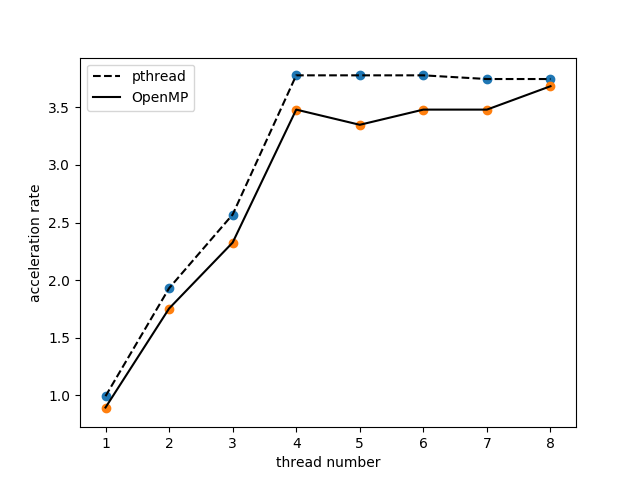
\includegraphics[width=0.8\linewidth]{ompTrend.png}
    \caption{加速比随线程数量变化}
    \label{fig:ompTrend}
\end{figure}
\par 而加速比随分块大小的变化如图\ref{fig:ompTrend2}所示,同样,实线为OpenMP实现,虚线为pthread实现。与随着线程变化的趋势一样,在同样的情况下OpenMP的性能比pthread性能低。在分块大小超过图片的1/2时更为明显,其下降趋势更为剧烈,推测是由于OpenMP的启动与初始化时间以及调度的分块引起的。
\par 从上述结果可以得出结论:在对于并行性能要求不是非常高时,使用OpenMP可以简化程序编写者的工作量,而使用pthread作出针对特定程序的并行算法则相对于OpenMP算法可以较大的提高程序的性能。
\begin{figure}[htpb]
    \centering
    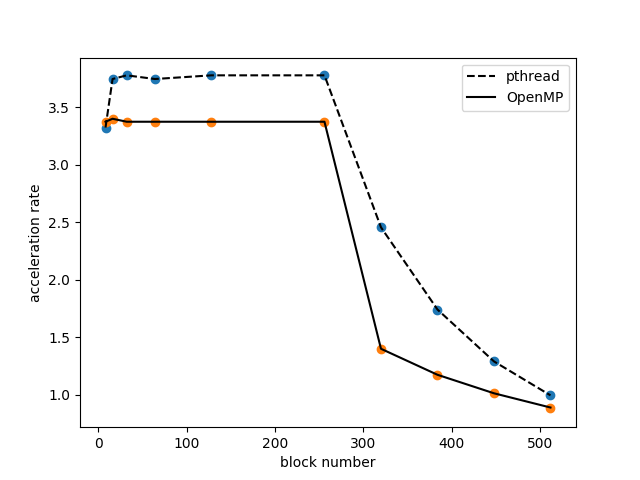
\includegraphics[width=0.8\linewidth]{ompTrend2.png}
    \caption{加速比随线分块大小变化}
    \label{fig:ompTrend2}
\end{figure}


